\documentclass[russian,utf8,12pt]{eskdtext}
\usepackage[numbertop, numbercenter]{eskdplain}

% - Подключаем шрифты из пакета scalable-cyrfonts-tex
\usepackage{cyrtimes}

% - Отступ красной строки
\setlength{\parindent}{1.25cm}

% - Убирает точку в списке литературы
\makeatletter
\def\@biblabel#1{#1 }

% - Точки для всех пунктов в оглавлении
\renewcommand*{\l@section}{\@dottedtocline{1}{1.5em}{2.3em}}
\renewcommand*{\l@subsection}{\@dottedtocline{1}{1.5em}{2.3em}}
\renewcommand*{\l@subsubsection}{\@dottedtocline{1}{1.5em}{2.3em}}

% - Для переопределения списков
\renewcommand{\theenumi}{\arabic{enumi}}
\renewcommand{\labelenumi}{\theenumi)}
\makeatother

\usepackage{enumitem}
\setlist{nolistsep, itemsep=0.3cm,parsep=0pt}

% - ГОСТ списка литературы
\bibliographystyle{utf8gost705u}

% - Верикальные отступы заголовков 
\ESKDsectSkip{section}{1em}{1em}
\ESKDsectSkip{subsection}{1em}{1em}
\ESKDsectSkip{subsubsection}{1em}{1em}

% - Изменение заголовков
\usepackage{titlesec}
\titleformat{\section}{\centering\normalfont\normalsize}{\thesection}{1.0em}{}
\titleformat{\subsection}{\centering\normalfont\normalsize}{\thesubsection}{1.0em}{}
\titleformat{\subsubsection}{\centering\normalfont\normalsize}{\thesubsubsection}{1.0em}{}
\titleformat{\paragraph}{\centering\normalsize}{\theparagraph}{1.0em}{}

% - Оставим место под ТЗ 
%\setcounter{page}{4}

% - Для больших таблиц
\usepackage{longtable}
\usepackage{tabularx}
\renewcommand{\thetable}{\thesection.\arabic{table}}

% - Используем графику в документе
\usepackage{graphicx}
\graphicspath{{images/}}
\renewcommand{\thefigure}{\thesection.\arabic{figure}}

% - Счётчики
\usepackage{eskdtotal}

% - Выравнивание по ширине
\sloppy

% - Разрешить перенос двух последних букв слова
\righthyphenmin=2

\RequirePackage{enumitem}
\renewcommand{\alph}[1]{\asbuk{#1}}
\setlist{nolistsep}
\setitemize[1]{label=--, fullwidth, itemindent=\parindent, 
  listparindent=\parindent}% для дефисного списка
\setenumerate[1]{label=\arabic*), fullwidth, itemindent=\parindent, 
  listparindent=\parindent}% для нумерованного списка
\setenumerate[2]{label=\alph*), fullwidth, itemindent=\parindent, 
  listparindent=\parindent, leftmargin=\parindent}% для списка 2-ой ступени, который будет нумероваться а), б) и т.д.

\usepackage{listings}  
\lstset{basicstyle=\ttfamily\small}

\begin{document}

\newpage
\ESKDthisStyle{empty}

\begin{center}
 Министерство образования и науки Российской Федерации\\
 Федеральное государственное бюджетное образовательное учреждение высшего профессионального образования\\
 <<ТОМСКИЙ ГОСУДАРСТВЕННЫЙ УНИВЕРСИТЕТ СИСТЕМ УПРАВЛЕНИЯ И РАДИОЭЛЕКТРОНИКИ>> (ТУСУР)\\
 Кафедра комплексной информационной безопасности электронно-вычислительных систем (КИБЭВС)\\
\end{center}

\vfill

\begin{flushright}
\begin{minipage}{0.45\textwidth}
 \begin{flushleft}
  УТВЕРЖДАЮ\\
  заведующий каф. КИБЭВС
  \underline{\hspace{3cm}}А.А. Шелупанов \\
  <<\underline{\hspace{1cm}}>>\underline{\hspace{3cm}}2015г.\\
 \end{flushleft}
\end{minipage}
\end{flushright}

\vfill

\begin{center}
ПРОЕКТИРОВАНИЕ, РАЗРАБОТКА БАЗЫ ДАННЫХ И ПРОГРАММНОГО ОБЕСПЕЧЕНИЯ ДЛЯ ЭЛЕКТРОННОЙ РЕГИСТРАЦИИ НА ПРИЕМ К ВРАЧУ 
(ЭЛЕКТРОННАЯ РЕГИСТРАТУРА)

Курсовая работа по дисциплине <<Безопасность систем баз данных>>

Пояснительная записка к курсовой работе
\end{center}

\vfill
\begin{flushright}
\begin{minipage}{0.45\textwidth}
 \begin{flushleft}
  Выполнила: \\
  студентка гр. 722 \\
  \underline{\hspace{3cm}}М.В. Мейта \\
  <<\underline{\hspace{1cm}}>>\underline{\hspace{3cm}}2015г.\\
 \end{flushleft}
\end{minipage}
\end{flushright}

\vfill

\begin{flushright}
\begin{minipage}{0.45\textwidth}
 \begin{flushleft}
  Научный руководитель: \\
  аспирант каф. КИБЭВС \\
  \underline{\hspace{3cm}}И.В. Горбунов \\
  <<\underline{\hspace{1cm}}>>\underline{\hspace{3cm}}2015г.\\
 \end{flushleft}
\end{minipage}
\end{flushright}

\vfill

\begin{center}
 Томск 2015
\end{center}

\newpage
\ESKDthisStyle{empty}
\paragraph{\hfill РЕФЕРАТ \hfill}
Курсовая работа содержит \ESKDtotal{page} страниц, \ESKDtotal{figure} рисунка, \ESKDtotal{table} таблицы, \ESKDtotal{bibitem} источников, \ESKDtotal{appendix} приложение.

БАЗЫ ДАННЫХ, SQLITE, MONODEVELOP, C#, GTKSharp.

Цель работы --- проектирование, разработка базы данных и клиентской части программного обеспечения для электронной регистрации на прием к врачу (электронная регистратура).

Задачей, поставленной на данный семестр, стало написание программного комплекса, имеющего следующие возможности: 
\begin{enumerate}
\item сбор и анализ событий системных журналов операционной системы;
\item сбор и анализ информации из журналов истории браузеров;
\item сбор и анализ истории переписки мессенджеров;
\item сбор и анализ событий журнальных файлов приложений;
\item поиск файлов по имени.
\end{enumerate}
Результатами работы в данном семестре являются:

\begin{itemize}
\item разработка архитектуры проекта;
\item использование в разработке системы контроля версий GIT;
\item использование Qt --- кроссплатформенной библиотеки С++;
\item изучение вопроса сертификации для возможности внедрения данного комплекса в гос. структуры, занимающиеся информационной безопасностью;
\item использование системы компьютерной вёрстки \TeX для написания документации.
\end{itemize}


Пояснительная записка выполнена при помощи системы компьютерной вёрстки \LaTeX.


\newpage
\ESKDstyle{plain}
\tableofcontents

\newpage
\ESKDstyle{plain}
\addcontentsline{toc}{section}{ТЕХНИЧЕСКОЕ ЗАДАНИЕ}
\ESKDthisStyle{empty}
\ESKDthisStyle{empty}

\begin{center}
 Министерство образования и науки Российской Федерации\\
 Федеральное государственное бюджетное образовательное учреждение высшего профессионального образования\\
 <<ТОМСКИЙ ГОСУДАРСТВЕННЫЙ УНИВЕРСИТЕТ СИСТЕМ УПРАВЛЕНИЯ И РАДИОЭЛЕКТРОНИКИ>> (ТУСУР)\\
 Кафедра комплексной информационной безопасности электронно-вычислительных систем (КИБЭВС)\\
\end{center}

\vfill


\begin{flushleft}
\begin{minipage}{0.45\textwidth}
 \begin{flushleft}
  УТВЕРЖДАЮ\\
  Заведующий каф. КИБЭВС, \\
  доктор технических наук, профессор \\
  \underline{\hspace{3cm}}А.А. Шелупанов \\
  <<\underline{\hspace{1cm}}>>\underline{\hspace{3cm}}2015г.\\
 \end{flushleft}
\end{minipage}
\hfill
\begin{minipage}{0.45\textwidth}
 \begin{flushleft}
  УТВЕРЖДАЮ\\
  Руководитель группы, \\
  студентка гр. 722 \\
  \underline{\hspace{3cm}}М.В. Мейта \\
  <<\underline{\hspace{1cm}}>>\underline{\hspace{3cm}}2015г.\\
 \end{flushleft}
\end{minipage}
\end{flushleft}

\vfill

\begin{center}
ПРОЕКТИРОВАНИЕ, РАЗРАБОТКА БАЗЫ ДАННЫХ И ПРОГРАММНОГО ОБЕСПЕЧЕНИЯ ДЛЯ ЭЛЕКТРОННОЙ РЕГИСТРАЦИИ НА ПРИЕМ К ВРАЧУ 
(ЭЛЕКТРОННАЯ РЕГИСТРАТУРА)

Курсовая работа по дисциплине <<Безопасность систем баз данных>>

ТЕХНИЧЕСКОЕ ЗАДАНИЕ

на \pageref{lastpage} листах

Действует с 1.03.2015
\end{center}

\vfill

\begin{flushleft}
\begin{minipage}{0.45\textwidth}
 \begin{flushleft}
  СОГЛАСОВАНО \\
  аспирант каф. КИБЭВС \\
  \underline{\hspace{3cm}}Горбунов И.В. \\
  <<\underline{\hspace{1cm}}>>\underline{\hspace{3cm}}2015г.\\
 \end{flushleft}
\end{minipage}
\end{flushleft}

\vfill

\begin{center}
 Томск 2015
\end{center}


\titleformat{\section}{\normalfont\normalsize}{\thesection}{1.0em}{}
\titleformat{\subsection}{\normalfont\normalsize}{\thesubsection}{1.0em}{}
\titleformat{\subsubsection}{\normalfont\normalsize}{\thesubsubsection}{1.0em}{}

\newpage
\section{Общие сведения}
\subsection{Полное наименование системы и ее условное обозначение}

Полное название программы: <<Электронная регистратура>>.

Условное обозначение: <<hospital\_register>>.


\subsection{Наименование предприятий (объединений) разработчика и заказчика (пользователя) системы и их реквизиты}

Разработчик: студентка гр.722 ФБ ТУСУРа: Мейта Марина Валерьевна.

Заказчик: Томский государственный университет систем управления и радиоэлектроники (ТУСУР), факультет безопасности (ФБ), в лице аспиранта кафедры комплексной информационной безопасности электронно-вычислительных систем (КИБЭВС) Горбунова И. В.

\subsection{Требования, на основании которых создается система, и даты их утверждения}

Задание на выполнение курсового проекта по дисциплине <<Безопасность систем баз данных>> утверждено Горбуновым И. В. 1 марта 2015 г.

\subsection{Плановые сроки начала и окончания работы по созданию системы}

Дата начала работы --- 1 марта 2015 года, дата окончания работы --- 1 июня 2015 года. 

\subsection{Сведения об источниках и порядке финансирования работ}

Финансирование осуществляется лицами, заинтересованными в разработке программного средства, а именно разработчиком из собственных средств.

\subsection{Прядок оформления и предъявления заказчику результатов работ по созданию системы (ее частей), по изготовлению и наладке отдельных средств (технических, программных, информационных) и программно-технических (программно-методических) комплексов системы}

Предоставляется промежуточная отчетность по завершении каждого установленного заказчиком этапа разработки. 
Документы предъявляются на бумажных носителях и в электронном виде не позднее установленных сроков. Этапы и сроки сдачи отчетности приведены в таблице~\ref{tab_1:tab_1}.

\begin{table}[ht]
\caption{Этапы разработки}
\label{tab_1:tab_1}
\begin{center}
\begin{tabularx}{\linewidth}{|X|X|X|}
\hline
Содержание этапа & Сроки & Отчетный документ \\
\hline
Подготовительный этап. Постановка задачи, сбор и анализ требований к разработке, проработка прототипа ПО, проработка прототипа БД.Разработка технического задания. & 1.03 --- 21.03 & Техническое задание. Прототипы ПО и БД. \\
\hline
Проектирование & 21.03 --- 14.04 & Технический проект. Пересмотренные прототипы. ПО и БД.  \\
\hline
Реализация спроектированного приложения и базы данных. Написание программной справки. Тестирование. & 14.04 --- 02.05 & Версия программного продукта. \\
\hline
Определение соответствия, разработанного ПО заданным критериям качества. & 02.05 --- 21.05 & Версия программного продукта.Результаты исследований. Результаты тестирования.\\
\hline
Оформление пояснительной записки. Прием работы. & 21.05 --- 01.05 & Пояснительная записка. \\
\hline
\end{tabularx}
\end{center}
\end{table}




\section{Назначение и цели создания (развития) системы}
\subsection{Назначение системы}

Программное обеспечение предназначено для работы с базой данных, содержащей в себе информацию, необходимую для электронной регистрации в поликлинике.

\subsection{Цели создания системы}

Поставлены следующие цели: уменьшить ожидаение в очередях к столу регистрации в поликлинике, облегчить процесс регистрации пациентов, обеспечить возможность просматривать и добавлять информацию о сотрудниках (врачах) и вносить изменения в расписание приемов.


\section{Характеристика объектов автоматизации}
\subsection{Краткие сведения об объекте автоматизации или ссылки на документы, содержащие такую информацию}

Объектом автоматизации является база данных, к которой обращается программное обеспечение за чтением или записью данных.


\section{Требования к системе}
\subsection{Общие требования к системе}
\subsubsection{Входные и выходные данные}

Входные данные:

В программе <<hospital\_register>> возможны следующие входные данные:
Ф.И.О. сотрудника, специальность сотрудника, день записи, серия и номер паспорта пациента, номер кабинета, день недели, ID сотрудника, начало и конец смены сотрудника, ID пациента, ID расписания и ID талона, Ф.И.О. пациента, день рождения пациента, месяц рождения пациента, год рождения пациента, пол пациента, код подразделения, адрес места жительства пациента, серия полиса пациента, номер полиса пациента, страховая компания.
Далее приведен диапазон допустимых значений. Все входные значения не должны быть пустыми (NULL).

В главном окне программы MainWindow возможен только один входной параметр --- пароль администратора. На него заведомо накладывается только одно ограничение --- пароль не должен быть пустой строкой.

В окне управления базой AdminWindow входные параметры следующие: Ф.И.О. сотрудника, специальность сотрудника, номер кабинета, день недели, ID сотрудника, начало и конец смены сотрудника, ID пациента, ID расписания и ID талона (таблица~\ref{tab:tab_1}). 

\begin{table}[ht]
\caption{Таблица признаков для AdminWindow}
\label{tab:tab_1}
\begin{center}
\begin{tabularx}{\linewidth}{|X|X|X|}
\hline
 Наименование признака & Описание признака & Диапазон допустимых значений\\
\hline
 employee\_name & Ф.И.О. сотрудника & Символы русского или латинского алфавита\\
\hline
 speciality & Специальность сотрудника & Символы русского или латинского алфавита\\
\hline
 office\_number & Номер кабинета сотрудника & 3 цифры от 0 до 9\\
\hline
 week\_day & День недели & Одно из заранее определенных значений (<<Пн>>, <<Вт>>, <<Ср>>, <<Чт>>, <<Пт>>, <<Сб>>, <<Вс>>)\\
\hline
 employee\_id & Идентификатор сотрудника & 10 цифр от 0 до 9 \\
\hline
 patient\_id & Идентификатор пациента & 10 цифр от 0 до 9 \\
\hline
 timetable\_id & Идентификатор расписания & 10 цифр от 0 до 9 \\
\hline
 talon\_id & Идентификатор талона & 10 цифр от 0 до 9 \\
\hline
 shift\_begining & Начало смены сотрудника & Строка формата <<ЧЧ:ММ>>, где ЧЧ (часы) и ММ (минуты) --- цифры от 0 до 9 \\
\hline
 shift\_ending & Конец смены сотрудника & Строка формата <<ЧЧ:ММ>>, где ЧЧ (часы) и ММ (минуты) --- цифры от 0 до 9\\
\hline
\end{tabularx}
\end{center}
\end{table}

В окне для записи на прием к врачу EnrollWindow входные параметры: Ф.И.О. сотрудника, специальность сотрудника, день записи, серия и номер паспорта пациента (таблица~\ref{tab:tab_2}). 

\begin{table}[ht]
\caption{Таблица признаков для EnrollWindow}
\label{tab:tab_2}
\begin{center}
\begin{tabularx}{\linewidth}{|X|X|X|}
\hline
 Наименование признака & Описание признака & Диапазон допустимых значений\\
\hline
 employee\_name & Ф.И.О. сотрудника & Одно из заранее определенных значений\\
\hline
 speciality & Специальность сотрудника & Одно из заранее определенных значений\\
\hline
 week\_day & День записи & Одно из заранее определенных значений (<<Пн>>, <<Вт>>, <<Ср>>, <<Чт>>, <<Пт>>, <<Сб>>, <<Вс>>)\\
\hline
 passport & Серия пасспорта пациента & 4 цифры от 0 до 9 \\
\hline
 passport & Номер паспорта пациента & 6 цифр от 0 до 9 \\
\hline
\end{tabularx}
\end{center}
\end{table}

В окне регистрации пациента PatientRegisterWindow входные параметры: Ф.И.О. пациента, день рождения пациента, месяц рождения пациента, год рождения пациента, пол пациента, серия паспорта пациента, номер паспорта пациента, код подразделения, адрес места жительства пациента, серия полиса пациента, номер полиса пациента, страховая компания (таблица~\ref{tab:tab_3}). 

\begin{table}[ht]
\caption{Таблица признаков для EnrollWindow}
\label{tab:tab_3}
\begin{center}
\begin{tabularx}{\linewidth}{|X|X|X|}
\hline
 Наименование признака & Описание признака & Диапазон допустимых значений\\
\hline
 patient\_name & Ф.И.О. сотрудника & Символы русского или латинского алфавита\\
\hline
 birth\_date & День рождения пациента & Число от 1 до 31\\
\hline
 birth\_date & Месяц рождения пациента & Одно из заранее определенных значений\\
\hline
 birth\_date & Год рождения пациента & Число от 1900 до 2020\\
\hline
 sex & Пол пациента & Одно из заранее определенных значений (<<М>> или <<Ж>>)\\
\hline
 passport & Серия пасспорта пациента & 4 цифры от 0 до 9 \\
\hline
 passport & Номер паспорта пациента & 6 цифр от 0 до 9 \\
\hline
 issue\_date & День выдачи паспорта & Число от 1 до 31\\
\hline
 issue\_date & Месяц выдачи паспорта & Одно из заранее определенных значений\\
\hline
 issue\_date & Год выдачи паспорта & Число от 1900 до 2020\\
\hline
 policy & Серия полиса пациента & 5 цифр от 0 до 9 \\
\hline
 policy & Номер полиса пациента & 6 цифр от 0 до 9 \\
\hline
 insurance\_agency & Название страховой медицинской компании & Символы русского или латинского алфавита \\
\hline
\end{tabularx}
\end{center}
\end{table}

\clearpagepage


Выходные данные:

Выходные данные сохраняются в PDF-файл <<talon.pdf>> в рабочей директории программы. Данный файл в дальнейшем может быть распечатан терминалом при завершении операции записи пациента. 

В файл <<talon.pdf>> выводятся следующие данные: Ф.И.О. врача, специальность, номер кабинета, рабочие часы, дата и день недели, Ф.И.О. пациента и страховой медицинский полис пациента.


\clearpage
\subsubsection{Требования к транспортированию и хранению}

Программа поставляется на CD, который должен быть помещен в жесткий футляр, обеспечивающий длительное хранение в отапливаемых помещениях в условиях, пригодных для хранения оптических дисков.
При транспортировании и хранении программного изделия должна быть предусмотрена защита от попадания пыли и атмосферных осадков. Климатические условия транспортирования:

\begin{itemize}
  \item температура окружающего воздуха, °С – от 5 до 50;
  \item атмосферное давление, кПа – 84,0-106,7;
  \item относительная влажность воздуха при 25 °С – 45-80\%.
\end{itemize}

\subsubsection{Требования к информационной и программной совместимости}

Программное обеспечение <<hospital\_register>> с ОС Linux Ubuntu/Debian.

Минимальные системные требования:

\begin{itemize}
  \item ОС Linux Ubuntu/Debian;
  \item процессор x86-архитектуры;
  \item объем ОЗУ для выполнения программы: не менее 300 Мб;
  \item объём видеопамяти: не менее 300 Мб;
  \item память на жестком диске: не менее 100 Мб для файлов БД и программы;
  \item монитор с разрешением 800x600 или выше;
  \item мышь, клавиатура;
  \item устройство для чтения CD;
  \item принтер.
\end{itemize}

\subsubsection{Требования к надежности}

При условии соблюдения требований эксплуатации и при контроле входных и выходных данных программа должна безотказно выполнять функции, определенные настоящим техническим заданием.

Время восстановления после отказа, вызванного сбоем технических средств, сбоем операционной системы, не должно превышать времени, необходимого на перезагрузку операционной системы и запуск программы.

Время восстановления после отказа, вызванного неисправностью технических средств, жестким сбоем операционной системы, не должно превышать времени, требуемого на устранение неисправностей технических средств и переустановки программных средств.

\subsubsection{Требования к эргономике и технической эстетике}

Взаимодействие пользователя с программой должно осуществляться посредством визуального графического интерфейса. Использование манипулятора типа <<мышь>>, клавиатуры. Элементы интерфейса должны быть схожими со стандартными элементами интерфейса приложений операционной системы. 

\subsubsection{Требования к эксплуатации}

Требования к помещениям, где эксплуатируются компьютеры, на которых предполагается работа системы, к микроклимату, акустическим шумам и вибрациям, освещению, организации и оборудованию рабочих мест определены санитарно-эпидемиологическими правилами и нормативами СанПиН 2.2.2/2.4.1340-03 <<Гигиенические требования к персональным электронно-вычислительным машинам и организации работы>>.

\subsubsection{Требования к маркировке и упаковке}

Программа поставляется в виде программного изделия на внешнем оптическом носителе (CD). 
Упаковка должна обеспечить защиту носителя от пыли и небольших механических повреждений (царапин). Упаковкой служит жесткий футляр с указанием названия программного продукта.

\subsection{Требования к функциям (задачам), выполняемым системой}
\subsubsection{Требования к составу выполняемых функций}

Программа должна считывать вводимые пользователям значения, выводить результаты запросов и генерировать талоны в формате PDF. При ошибочных действиях пользователя, связанных с вводом данных или ошибками при обращении к БД, программа должна уведомлять пользователя об ошибке.

\subsection{Требования к видам обеспечения}
\subsubsection{Требования к техническому обеспечению системы}

Для работы системы требуется компьютер, на котором функционирует операционная система OC Linux Ubuntu/Debian. Для работы программы необходимы:

\begin{itemize}
  \item процессор x86-архитектуры;
  \item объем ОЗУ для выполнения программы: не менее 300 Мб;
  \item объём видеопамяти: не менее 300 Мб;
  \item память на жестком диске: не менее 100 Мб для файлов БД и программы;
  \item монитор с разрешением 800x600 или выше;
  \item мышь, клавиатура;
  \item устройство для чтения CD;
  \item принтер.
\end{itemize}

\subsubsection{Требования к информационной и программной совместимости}

Работа приложения гарантируется в OC Linux Ubuntu/Debian.



\newpage
\section{Состав и содержание работ по созданию системы}
\input{tz/tz_5}

\section{Порядок контроля и приема системы}
\subsection{Виды, состав, объем и методы испытаний системы и ее составных частей (виды испытаний в соответствии с действующими нормами, распространяющимися на разрабатываемую систему)}

Текущий подход к контролю качества подразумевает следующие этапы проекта:
\begin{itemize}
  \item подсистема готова к демонстрации заказчику;
  \item подсистема готова к эксплуатации.
\end{itemize}

\subsection{Общие требования к приему работ по стадиям (перечень участвующих предприятий и организаций, место и сроки проведения), порядок согласования и утверждения приемочной документации}

Прием работ по стадиям осуществляется проверкой отчетных документов по стадиям.

\subsection{Статус приемной комиссии (государственная, межведомственная, ведомственная)}

Кафедральная комиссия. Состав комиссии --- научный руководитель: аспирант кафедры КИБЭВС Горбунов И. В.


\section{Требования к составу и содержанию работ по подготовке объекта автоматизации к вводу системы в действие}
Для работы с системой необходимо переместить директорию программы с CD на жесткий диск компьютера, 

\textbf{ПОПРАВИТЬ!!!!!}


\section{Требования к документированию}
\input{tz/tz_8}

\section{Источники разработки}
\begin{enumerate}
  \item \textbf{ПОПРАВИТЬ!!!!!}
  \item 
  \item 
\end{enumerate}


\newpage
\begin{center}
  РАЗРАБОТАНО
\end{center}

\begin{table}[ht]
\label{tab:developed}
\begin{center}
\begin{tabularx}{\linewidth}{|X|X|X|X|X|}
\hline
Наименование организации, предприятия & Должность исполнителя & Ф.И.О. & Подпись & Дата\\
\hline
ТУСУР Каф. КИБЭВС & Руководитель проекта, документатор, программист & Мейта М.В. & & <<\_\_>>\_\_\_\_\_2015 г. \\
\hline
\end{tabularx}
\end{center}
\end{table}

\begin{center}
  СОГЛАСОВАНО
\end{center}

\begin{table}[ht]
\label{tab:agreed}
\begin{center}
\begin{tabularx}{\linewidth}{|X|X|X|X|X|}
\hline
Наименование организации, предприятия & Должность исполнителя & Ф.И.О. & Подпись & Дата\\
\hline
ТУСУР Каф. КИБЭВС & Аспирант каф. КИБЭВС & Горбунов И. В. & & <<\_\_>>\_\_\_\_\_2015 г. \\
\hline
\end{tabularx}
\end{center}
\end{table}


% - маркер для ссылки на страницу
\label{lastpage}


\titleformat{\section}{\centering\normalfont\normalsize}{\thesection}{1.0em}{}
\titleformat{\subsection}{\centering\normalfont\normalsize}{\thesubsection}{1.0em}{}
\titleformat{\subsubsection}{\centering\normalfont\normalsize}{\thesubsection}{1.0em}{}

\newpage
\ESKDstyle{plain}
\setcounter{section}{0}
\section*{ВВЕДЕНИЕ}
\addcontentsline{toc}{section}{ВВЕДЕНИЕ}
В качестве задания на курсовую работу была поставлена задача разработать базу данных и программу пользователя для осуществления электронной регистрации (записи на прием к врачу) в поликлинике.  


\newpage
\section{Проектирование инфологической модели данных}
\setcounter{figure}{0}
Инфологическая (концептуальная) модель предметной области представляет собой информационную модель наиболее высокого уровня абстракции и в сущности является как образом реальности, так и образом проектируемой базы данных для этой реальности. Она включает в себя описание информационных объектов или понятий предметной области и связей между ними. а также описание ограничений целостности, т.е. требований к допустимым значениям данных и к связям между ними.

Описание бизнесс-процессов в системе электронной регистрации пациентов представлено на диаграммах IDEF0, DFD IDEF3 (рисунки \ref{idef0_1:idef0_1}-\ref{idef3_2:idef3_2}).

\begin{figure}[h!]
\center{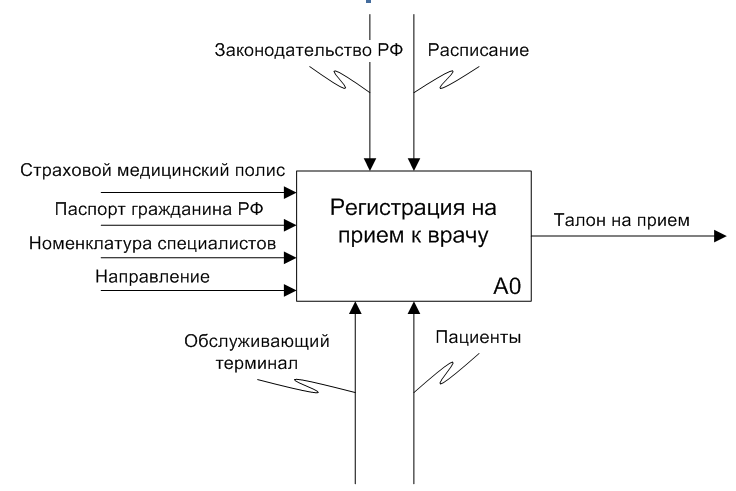
\includegraphics[width=0.5\linewidth]{idef0_1}}
\caption{<<Черный ящик>>}
\label{idef0_1:idef0_1}
\end{figure} 

\begin{figure}[h!]
\center{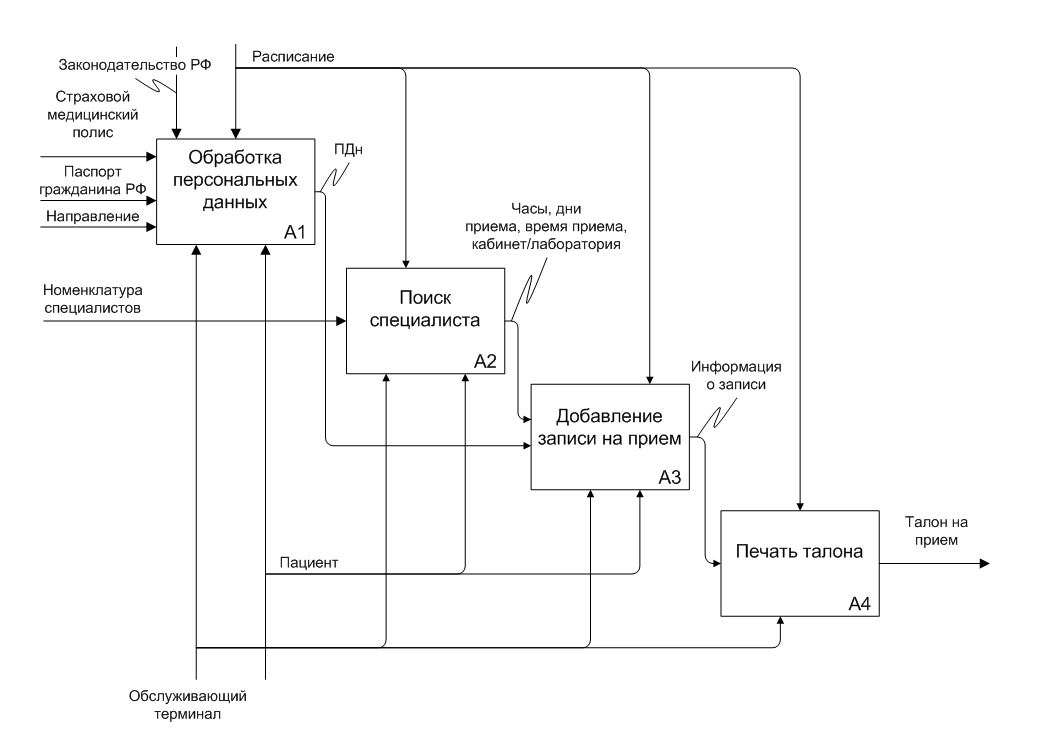
\includegraphics[width=0.9\linewidth]{idef0_2}}
\caption{Диаграмма IDEF0}
\label{idef0_2:idef0_2}
\end{figure} 

\begin{figure}[h!]
\center{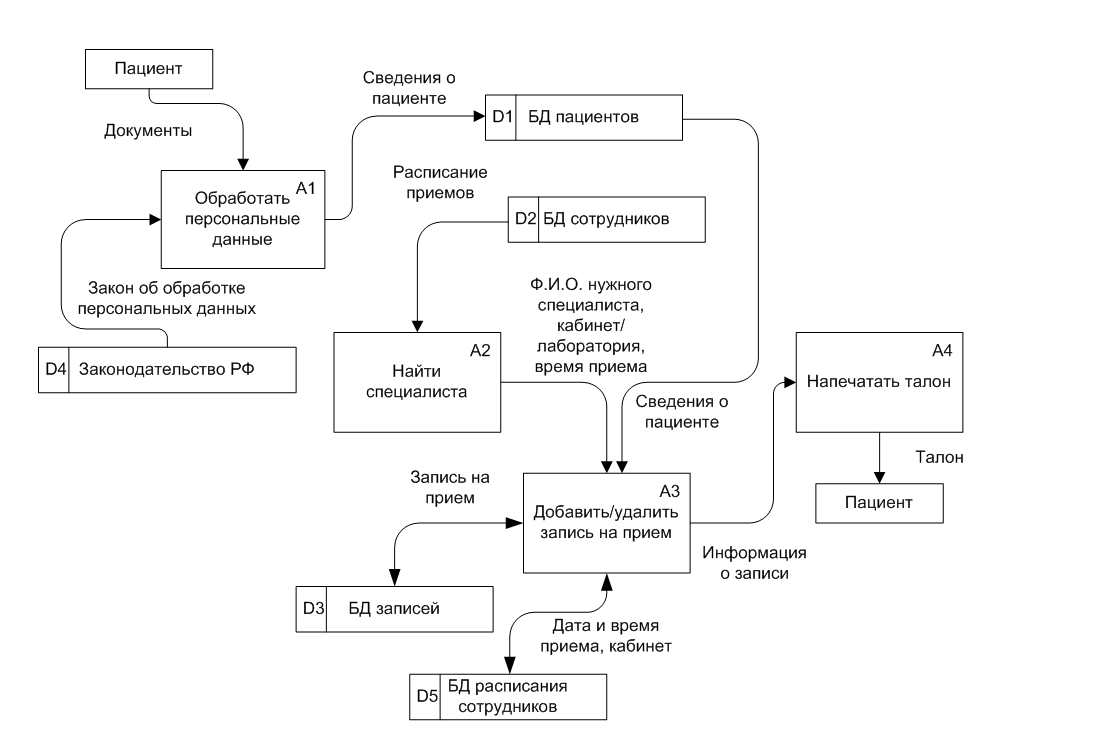
\includegraphics[width=0.9\linewidth]{dfd}}
\caption{DFD-диаграмма бизнес-процессов}
\label{dfd:dfd}
\end{figure} 

\begin{figure}[h!]
\center{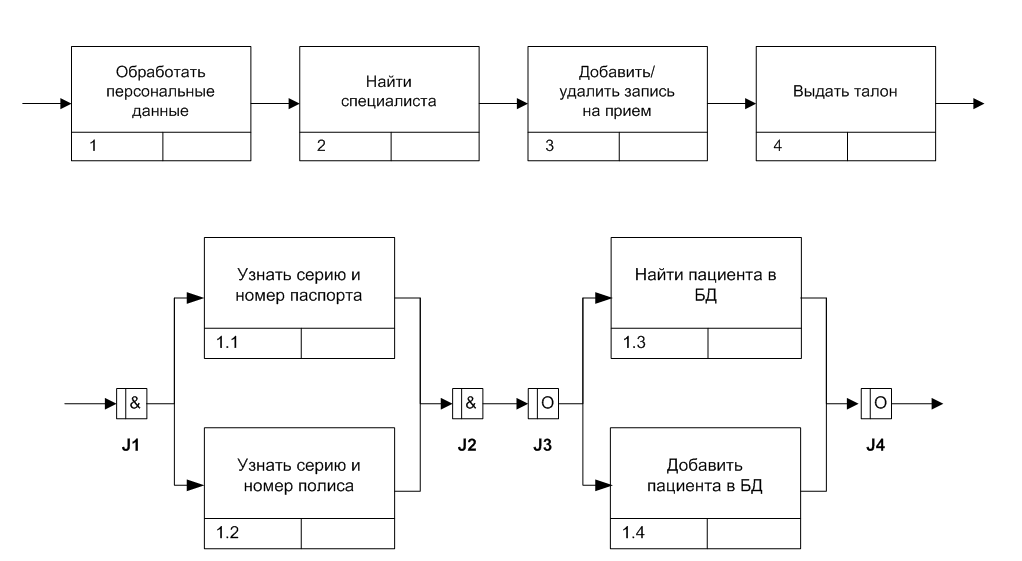
\includegraphics[width=0.9\linewidth]{idef3_1}}
\caption{Диаграмма IDEF3 (часть 1)}
\label{idef3_1:idef3_1}
\end{figure} 

\begin{figure}[h!]
\center{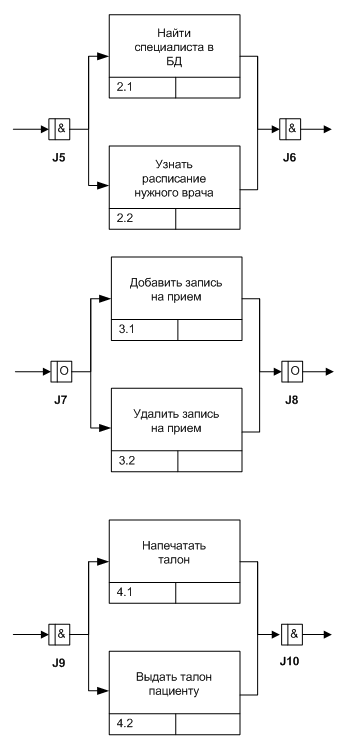
\includegraphics[width=0.4\linewidth]{idef3_2}}
\caption{Диаграмма IDEF3 (часть 2)}
\label{idef3_2:idef3_2}
\end{figure} 

\clearpage






\newpage
\section{Проектирование даталогической модели данных}
\setcounter{figure}{0}
Логическая (даталогическая) модель --- это схема базы данных на основе конкретной модели данных, набор схем отношений с указанием первичных ключей, а также «связей» между отношениями, представляющих собой внешние ключи.

Модель <<Сущность-связь>> (ER-модель) представлена на рисунке \ref{idef1x:idef1x}.

\begin{figure}[h!]
\center{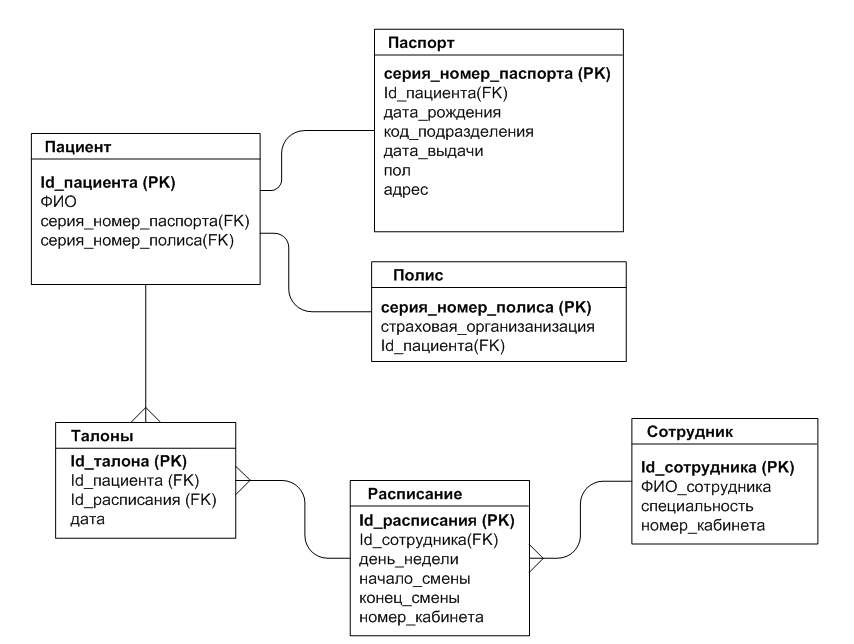
\includegraphics[width=0.9\linewidth]{idef1x}}
\caption{Диаграмма IDEF1X (модель <<Сущность-связь>>)}
\label{idef1x:idef1x}
\end{figure} 

\clearpage


\newpage
\section{Описание базы данных}
\setcounter{figure}{0}
В данном разделе рассмотрены ограничения, накладываемые на входные данные записей в различных таблицах проектируемой БД, типы входных данных и другие особенности содаваемых таблиц.

\subsection{Таблица <<patient>>}
Ограничения на таблицу <<patient>> (пациент):

\begin{itemize}
  \item ID пациента не меньше единицы;
  \item фамилия, имя отчество не должно превосходить 50 символов;
  \item ни один из атрибутов не дожен быть пустым (NULL).
\end{itemize}

\subsection{Таблица <<passport>>}
Ограничения на таблицу <<passport>> (паспорт):

\begin{itemize}
  \item ID пасспорта не меньше единицы;
  \item серия паспорта не должна превосходить 4 символа;
  \item номер паспорта не должен превосходить 6 символов;
  \item адрес места жительства не должен превосходить 100 символов;
  \item атрибут <<пол>> должен состоять из 1 символа (М/Ж);
  \item ни один из атрибутов не дожен быть пустым (NULL).
\end{itemize}

\subsection{Таблица <<policy>>}
Ограничения на таблицу <<policy>> (полис):

\begin{itemize}
  \item ID полиса не меньше единицы;
  \item название страховой медицинской компании не должно превосходить 100 символов;
  \item ни один из атрибутов не дожен быть пустым (NULL).
\end{itemize}

\subsection{Таблица <<talon>>}
Ограничения на таблицу <<talon>> (талон):

\begin{itemize}
  \item ID талона не меньше единицы;
  \item ни один из атрибутов не дожен быть пустым (NULL).
\end{itemize}

\subsection{Таблица <<timetable>>}
Ограничения на таблицу <<timetable>> (расписание):

\begin{itemize}
  \item ID расписания не меньше единицы;
  \item день недели должен состоять из 2-ух символов (<<Пн>>, <<Вт>> и т.д.);
  \item ни один из атрибутов не дожен быть пустым (NULL).
\end{itemize}

\subsection{Таблица <<employee>>}
Ограничения на таблицу <<employee>> (сотрудник):

\begin{itemize}
  \item ID сотрудника не меньше единицы;
  \item специальность сотрудника не должна превосходить 50 символов;
  \item фамилия, имя отчество не должно превосходить 50 символов;
  \item номер рабочего кабинета должен состоять из 3 символов;
  \item ни один из атрибутов не дожен быть пустым (NULL).
\end{itemize}

\subsection{Роли базы данных}
SQLite является встраиваемой реляционной базой данных и не использует парадигму <<клиент-сервер>>, то есть движок SQLite не является отдельно работающим процессом, с которым взаимодействует программа, а предоставляет библиотеку, с которой программа компонуется и движок становится составной частью программы. Таким образом, в качестве протокола обмена используются вызовы функций (API) библиотеки SQLite. Такой подход уменьшает накладные расходы, время отклика и упрощает программу. SQLite хранит всю базу данных (включая определения, таблицы, индексы и данные) в единственном стандартном файле на том компьютере, на котором исполняется программа.\cite{sqlitedoc}

В SQLite отсутствует разграничение ролей как таковых, поэтому потребовалось вводить меры по защите БД непосредственно в программном приложении для работы с базой. На уровне приложения были условно созданы 2 роли: <<администратор>> и <<пациент>>. <<Администратор>> при вводе пароля (хэш от пароля сравнивается с хэшем, хранимым в БД) получает доступ к программному изменению и просмотру данных в базе. <<Пациент>> имеет свободный доступ к форме для записи на прием и регистрации.

\subsection{Защита от SQL–инъекций}
Поскольку база данных SQLite является встраиваемой реляционной базой данных и представляет собой файл, провести SQL-инъекцию невозможно. Однако необходимо ограничить доступ к базе на уровне файловой системы, чтобы исключить возможность несанкционированного доступа (копирования, изменения, удаления данных или самой базы).


\clearpage
\section{Описание процесса деятельности} 
\setcounter{figure}{0}
\subsection{Постановка задачи}

База данных и программа <<hospital\_register>> создается для внедрения в поликлиниках в качестве электронной регистратуры.

\subsection{Описание данных программы}
\subsubsection{Входные данные}
В программе <<hospital\_register>> возможны следующие входные данные:
Ф.И.О. сотрудника, специальность сотрудника, день записи, серия и номер паспорта пациента, номер кабинета, день недели, ID сотрудника, начало и конец смены сотрудника, ID пациента, ID расписания и ID талона, Ф.И.О. пациента, день рождения пациента, месяц рождения пациента, год рождения пациента, пол пациента, код подразделения, адрес места жительства пациента, серия полиса пациента, номер полиса пациента, страховая компания.
Далее приведен диапазон допустимых значений. Все входные значения не должны быть пустыми (NULL).

В главном окне программы MainWindow возможен только один входной параметр --- пароль администратора. На него заведомо накладывается только одно ограничение --- пароль не должен быть пустой строкой.

В окне управления базой AdminWindow входные параметры следующие: Ф.И.О. сотрудника, специальность сотрудника, номер кабинета, день недели, ID сотрудника, начало и конец смены сотрудника, ID пациента, ID расписания и ID талона (таблица~\ref{tab:tab_1}). 

\begin{table}[ht]
\caption{Таблица признаков для AdminWindow}
\label{tab:tab_1}
\begin{center}
\begin{tabularx}{\linewidth}{|X|X|X|}
\hline
 Наименование признака & Описание признака & Диапазон допустимых значений\\
\hline
 employee\_name & Ф.И.О. сотрудника & Символы русского или латинского алфавита\\
\hline
 speciality & Специальность сотрудника & Символы русского или латинского алфавита\\
\hline
 office\_number & Номер кабинета сотрудника & 3 цифры от 0 до 9\\
\hline
 week\_day & День недели & Одно из заранее определенных значений (<<Пн>>, <<Вт>>, <<Ср>>, <<Чт>>, <<Пт>>, <<Сб>>, <<Вс>>)\\
\hline
 employee\_id & Идентификатор сотрудника & 10 цифр от 0 до 9 \\
\hline
 patient\_id & Идентификатор пациента & 10 цифр от 0 до 9 \\
\hline
 timetable\_id & Идентификатор расписания & 10 цифр от 0 до 9 \\
\hline
 talon\_id & Идентификатор талона & 10 цифр от 0 до 9 \\
\hline
 shift\_begining & Начало смены сотрудника & Строка формата <<ЧЧ:ММ>>, где ЧЧ (часы) и ММ (минуты) --- цифры от 0 до 9 \\
\hline
 shift\_ending & Конец смены сотрудника & Строка формата <<ЧЧ:ММ>>, где ЧЧ (часы) и ММ (минуты) --- цифры от 0 до 9\\
\hline
\end{tabularx}
\end{center}
\end{table}

В окне для записи на прием к врачу EnrollWindow входные параметры: Ф.И.О. сотрудника, специальность сотрудника, день записи, серия и номер паспорта пациента (таблица~\ref{tab:tab_2}). 

\begin{table}[ht]
\caption{Таблица признаков для EnrollWindow}
\label{tab:tab_2}
\begin{center}
\begin{tabularx}{\linewidth}{|X|X|X|}
\hline
 Наименование признака & Описание признака & Диапазон допустимых значений\\
\hline
 employee\_name & Ф.И.О. сотрудника & Одно из заранее определенных значений\\
\hline
 speciality & Специальность сотрудника & Одно из заранее определенных значений\\
\hline
 week\_day & День записи & Одно из заранее определенных значений (<<Пн>>, <<Вт>>, <<Ср>>, <<Чт>>, <<Пт>>, <<Сб>>, <<Вс>>)\\
\hline
 passport & Серия пасспорта пациента & 4 цифры от 0 до 9 \\
\hline
 passport & Номер паспорта пациента & 6 цифр от 0 до 9 \\
\hline
\end{tabularx}
\end{center}
\end{table}

В окне регистрации пациента PatientRegisterWindow входные параметры: Ф.И.О. пациента, день рождения пациента, месяц рождения пациента, год рождения пациента, пол пациента, серия паспорта пациента, номер паспорта пациента, код подразделения, адрес места жительства пациента, серия полиса пациента, номер полиса пациента, страховая компания (таблица~\ref{tab:tab_3}). 

\begin{table}[ht]
\caption{Таблица признаков для EnrollWindow}
\label{tab:tab_3}
\begin{center}
\begin{tabularx}{\linewidth}{|X|X|X|}
\hline
 Наименование признака & Описание признака & Диапазон допустимых значений\\
\hline
 patient\_name & Ф.И.О. сотрудника & Символы русского или латинского алфавита\\
\hline
 birth\_date & День рождения пациента & Число от 1 до 31\\
\hline
 birth\_date & Месяц рождения пациента & Одно из заранее определенных значений\\
\hline
 birth\_date & Год рождения пациента & Число от 1900 до 2020\\
\hline
 sex & Пол пациента & Одно из заранее определенных значений (<<М>> или <<Ж>>)\\
\hline
 passport & Серия пасспорта пациента & 4 цифры от 0 до 9 \\
\hline
 passport & Номер паспорта пациента & 6 цифр от 0 до 9 \\
\hline
 issue\_date & День выдачи паспорта & Число от 1 до 31\\
\hline
 issue\_date & Месяц выдачи паспорта & Одно из заранее определенных значений\\
\hline
 issue\_date & Год выдачи паспорта & Число от 1900 до 2020\\
\hline
 policy & Серия полиса пациента & 5 цифр от 0 до 9 \\
\hline
 policy & Номер полиса пациента & 6 цифр от 0 до 9 \\
\hline
 insurance\_agency & Название страховой медицинской компании & Символы русского или латинского алфавита \\
\hline
\end{tabularx}
\end{center}
\end{table}

\clearpagepage


\subsubsection{Выходные данные}
Выходные данные сохраняются в PDF-файл <<talon.pdf>> в рабочей директории программы. Данный файл в дальнейшем может быть распечатан терминалом при завершении операции записи пациента. 

В файл <<talon.pdf>> выводятся следующие данные: Ф.И.О. врача, специальность, номер кабинета, рабочие часы, дата и день недели, Ф.И.О. пациента и страховой медицинский полис пациента.













\clearpage
\subsection{Основные технические решения}
\subsubsection{Алгоритм}

Предварительного заполнения базы данных не требуется, однако для возможности добавления записи и регистрации пациента администратору сначала необходимо заполнить базу сотрудников и расписаний.

\begin{center}
  Шаг 1
\end{center}

При авторизации от имени пациента в главном окне программы (MainWindow) появится окно для записи на прием к врачу (EnrollWindow). Необходимо выбрать нужного специалиста, найти его расписание и правильно заполнить предлагаемую форму. Если входные значения были введены неверно, появится сообщение об ошибке. 

\begin{center}
  Шаг 2
\end{center}

Программа проверяет, есть ли уже в БД введенные пользователем серия и номер паспорта. Если данные о пациенте в базе уже есть и форма заполнена верно, появится сообщение об успешной записи, либо сообщение об ошибке записи, если такая запись уже была добавлена в БД.

\begin{center}
  Шаг 3
\end{center}

Если данных о пациенте в базе нет, то появится форма регистрации пациента (PatientRegisterWindow). Если все поля формы заполнены верно, пациент будет добавлен в базу и в окне записи на прием при повторной операции записи появится уведомление об успешном завершении операции, в результате которой будет сгенерирован PDF-файл (талон), готовый к печати.

\begin{center}
  Шаг 4
\end{center}

При авторизации от имени администратора программа сверяет хеш введённого пароля с  хешем, который хранится в БД. Если они совпадают, то открывается окно управления базой данных (AdminWindow), если нет, то появляется уведомление об ошибочной авторизации.

\begin{center}
  Шаг 5
\end{center}

Окно управления базой данных (AdminWindow) позволяет администратору просматривать, удалять и добавлять данные в базу. Для этого необходимо вводить корректные данные, в противном случае операции удаления и добавления выполняться не будут, появится сообщение об ошибке ввода или обращения к базе.

Блок-схема алгоритма работы программы представлена на рисунке~\ref{block:block}.

\begin{figure}[h!]
\center{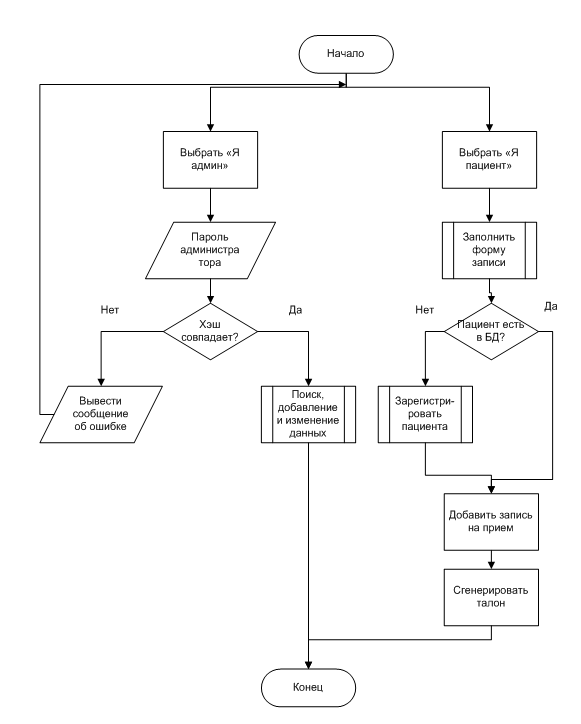
\includegraphics[width=0.8\linewidth]{block}}
\caption{Блок-схема алгоритма работы программы}
\label{block:block}
\end{figure}

\subsubsection{Численность, функции и квалификация персонала}

Для использования системы необходим администратор, который будет добавлять новых сотрудников и менять расписание уже добавленных, следить за целостностью системы, удалять ПДн пациентов по мере необходимости.

\subsubsection{Обеспечение потребительских характеристик системы}

Надежность обеспечивается путем следования стандартам написания кода и использования блоков try-catch для обработки исключительных ситуаций.
Производительность системы обеспечивается путем использования оптимальных алгоритмов.

\subsubsection{Функции, выполняемые системой}

Функциями, выполняемыми программой <<hospital\_register>>, являются регистрация пациентов, добавление записей на прием, печать талонов, управление расписанием и номенклатурой сотрудников (врачей), а также управление записями в БД. 

\subsubsection{Комплекс технических средств}

Для функционирования системы необходимы следующие аппаратные средства:

\begin{itemize}
  \item ОС Linux Ubuntu/Debian;
  \item процессор x86-архитектуры;
  \item объем ОЗУ для выполнения программы: не менее 300 Мб;
  \item объём видеопамяти: не менее 300 Мб;
  \item память на жестком диске: не менее 100 Мб для файлов БД и программы;
  \item монитор с разрешением 800x600 или выше;
  \item мышь, клавиатура;
  \item устройство для чтения CD;
  \item принтер.
\end{itemize}

\subsubsection{Информационное обеспечение системы}

Система поставляется с руководством пользователя и программиста.

\subsubsection{Программное обеспечение системы}

Система разворачивается на компьютере с ОС Linux Ubuntu/Debian.

\section{Мероприятия по подготовке персонала}

Провести ознакомление персонала с руководством пользователя.








\clearpage
\section{Руководство пользователя} 
\setcounter{figure}{0}
После запуска приложения в главном окне будет предложено осуществить вход от имени пользователя (рис.~\ref{main_win_patient:main_win_patient}) или администратора (рис.~\ref{main_window_admin:main_window_admin}).

\begin{figure}[h!]
\center{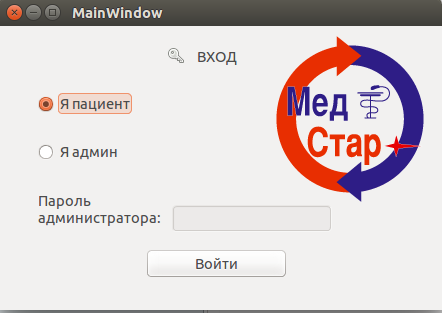
\includegraphics[width=0.5\linewidth]{main_win_patient}}
\caption{Вход от имени пользователя}
\label{main_win_patient:main_win_patient}
\end{figure}

\begin{figure}[h!]
\center{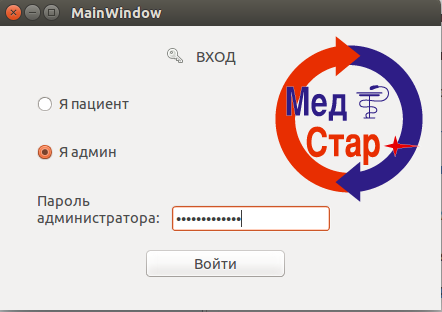
\includegraphics[width=0.5\linewidth]{main_window_admin}}
\caption{Вход от имени администратора}
\label{main_window_admin:main_window_admin}
\end{figure}
 
После нажатия кнопки <<Войти>> от лица пациента появится окно для записи на прием (рис.~\ref{enroll:enroll}). 
Если пациент еще не зарегистрирован в базе данных, то ему будет предложено пройти регистрацию (рис.~\ref{register_win:register_win}). После чего необходимо повторно нажать кнопку <<Записаться>> в окне для записи на прием. В результате будет успешно добавлен и сгенерирован в формате PDF талон на прием к специалисту (рис.~\ref{talon:talon}).

\begin{figure}[h!]
\center{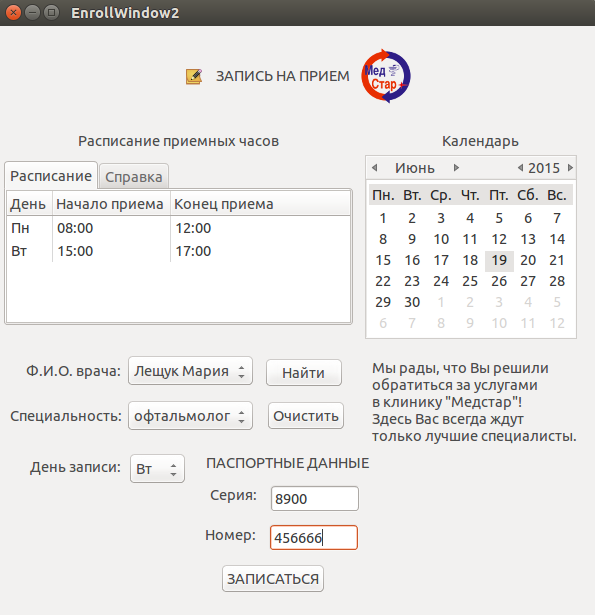
\includegraphics[width=0.9\linewidth]{enroll}}
\caption{Окно для записи на прием}
\label{enroll:enroll}
\end{figure}

\begin{figure}[h!]
\center{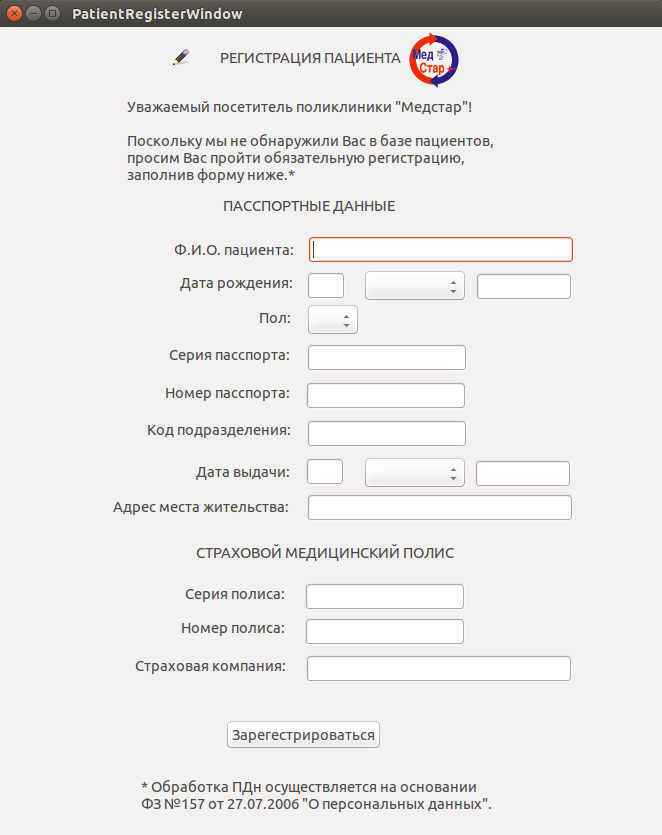
\includegraphics[width=0.9\linewidth]{register_win}}
\caption{Окно регистрации}
\label{register_win:register_win}
\end{figure}

\begin{figure}[h!]
\center{
\includegraphics[width=0.9\linewidth]{talon}}
\caption{Талон пациента}
\label{talon:talon}
\end{figure}

После нажатия кнопки <<Войти>> от лица администратора и успешного ввода пароля станет доступно окно управления базой данных. Оно позволяет как просматривать данные в таблицах (рис.~\ref{admin_find:admin_find}), так и добавлять (рис.~\ref{admin_insert:admin_insert}) и удалять их (рис.~\ref{admin_delete:admin_delete}) 

\begin{figure}[h!]
\center{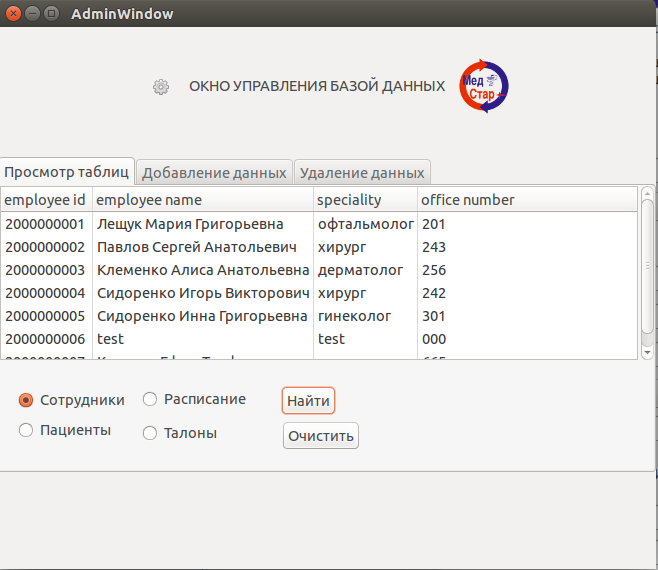
\includegraphics[width=0.9\linewidth]{admin_find}}
\caption{Просмотр данных в таблицах}
\label{admin_find:admin_find}
\end{figure}

\begin{figure}[h!]
\center{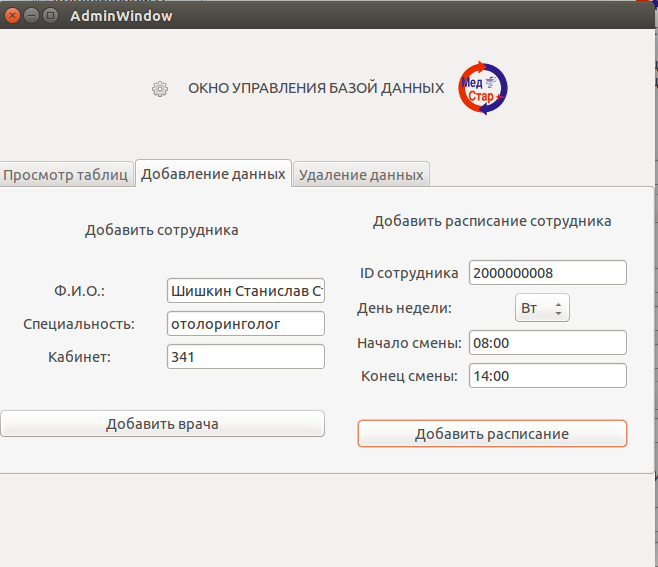
\includegraphics[width=0.9\linewidth]{admin_insert}}
\caption{Добавление данных}
\label{admin_insert:admin_insert}
\end{figure}

\begin{figure}[h!]
\center{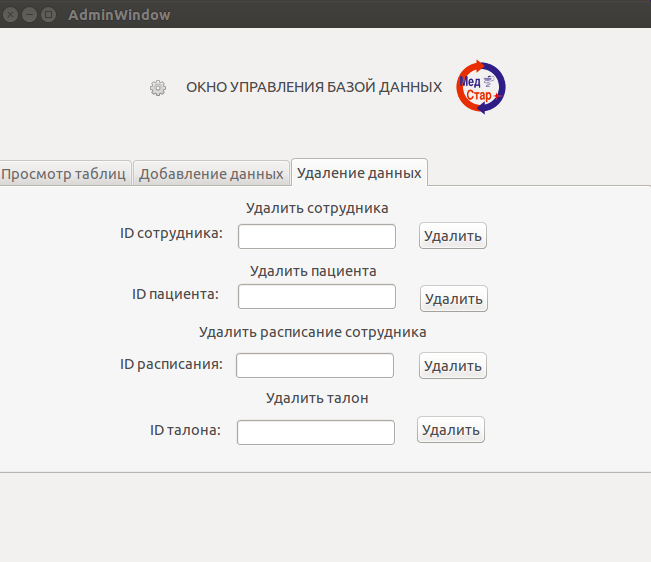
\includegraphics[width=0.7\linewidth]{admin_delete}}
\caption{Удаление данных}
\label{admin_delete:admin_delete}
\end{figure}

Необходимо правильно заполнять все поля для ввода. Если где-либо ввод осуществлен неверно, появится сообщение об ошибке ввода (рис.~\ref{err_win:err_win}), если же все действия проделаны верно --- сообщение об успешном завершении операции (рис.~\ref{suc_win:suc_win}).

\begin{figure}[h!]
\center{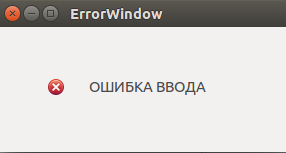
\includegraphics[width=0.5\linewidth]{err_win}}
\caption{Сообщение об ошибке ввода}
\label{err_win:err_win}
\end{figure}

\begin{figure}[h!]
\center{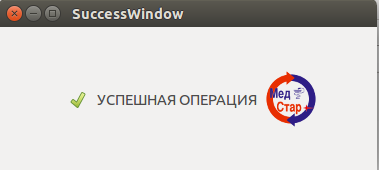
\includegraphics[width=0.5\linewidth]{suc_win}}
\caption{Сообщение об успешном завершении операции}
\label{suc_win:suc_win}
\end{figure}


\clearpage
\section{Руководство программиста} 
\setcounter{figure}{0}
\input{programmer_guide}


\clearpage
\section{Перспективы применения программы}
\setcounter{figure}{0}


% \section{Инструменты}
% \setcounter{figure}{0}
% \subsection{Система контроля версий Git}
% Для разработки программного комплекса для проведения компьютерной экспертизы решено использовать Git.

Git  — распределённая система управления версиями файлов. Проект был создан Линусом Торвальдсом для управления разработкой ядра Linux,  как противоположность  системе управления версиями Subversion (также известная как «SVN») \cite{progit}.

Необходимость использования системы версий, очевидна. Так как в группе несколько программистов и тестер, мы имеем:
\begin{itemize}
\item возможность удаленной работы с исходными кодами;
\item возможность создавать свои ветки, не мешая при этом другим разработчикам;
\item доступ к последним изменениям в коде, т.к. все исходники хранятся на сервере git.keva.su ;
\item исходные коды защищены, доступ к ним можно получить лишь имея RSA-ключ;
\item возможность откатиться к любой стабильной стадии проекта.
\end{itemize}

Основные постулаты работы с кодом в системе Git:

\begin{itemize}
\item каждая задача решается в своей ветке;
\item коммитим сразу, как что-то получили осмысленное;
\item в master мержится не разработчиком, а вторым человеком, который производит вычитку и тестирование изменения;
\item все коммиты должны быть осмысленно подписаны/прокомментированы.
\end{itemize}

Для работы над проектом нами был поднят собственный репозиторий на сервере git.keva.su.
Адреса репозиториев следующие:

Исходные файлы проекта:

git clone git@git.keva.su:gpo.git gpo.git

Репозиторий для тестирования проекта:

git clone git@git.keva.su:gpo-testdata.git gpo-testdata.git

% \subsection{Система компьютерной вёрстки \TeX}
% \TeX\ --- это созданная американским математиком и программистом Дональдом Кнутом система для вёрстки текстов. Сам по себе \TeX\ представляет собой специализированный язык программирования.Каждая издательская система представляет собой пакет макроопределений этого языка.

\LaTeX\ --- это созданная Лэсли Лэмпортом издательская система на базе \TeX'а\cite{lvovskyi}. \LaTeX\ позволяет пользователю сконцентрировать свои услия на содержании и структуре текста, не заботясь о деталях его оформления.

Для подготовки отчётной и иной документации нами был выбран \LaTeX\, так как совместно с системой контроля версий Git он предоставляет возможность совместного создания и редактирования документов. Огромным достоинством системы \LaTeX\ то, что создаваемые с её помощью файлы обладают высокой степенью переносимости \cite{latexrus}.

Совместно с \LaTeX\ часто используется Bib\TeX\ --- программное обеспечение для создания форматированных списков библиографии. Оно входит в состав дистрибутива \LaTeX\ и позволяет создавать удобную, универсальную и долговечную библиографию. Bib\TeX\ стал одной из причин, по которой нами был выбран \LaTeX\ для создания документации.

% \section{Технические характеристики}
% \subsection {Требования к аппаратному обеспечению}

Минимальные системные требования:

\begin{itemize}
\item процессор 1ГГц Pentium 4;
\item оперативная память 512 Мб;
\item место на жёстком диске -- 9 Гб.
\end{itemize}

\subsection {Требования к программному обеспечению}
Для корректной работы разрабатываемого программного комплекса на компьютере должна быть установлена операционная система Debian Squeeze или выше, данная система должна иметь набор библиотек QT.




\newpage
\section*{ЗАКЛЮЧЕНИЕ}
\addcontentsline{toc}{section}{ЗАКЛЮЧЕНИЕ}
В дальнейшем программу следует доработать следующим образом:
сконфигурировать и отладить решение для успешного запуска программы на ОС Windows, добавить автоматический вывод на печать сгенерированного талона, доработать адаптивный интерфейс программы (изменить контейнеры в GTK-окнах), оптимизировать программный код. Можно также расширить возможности программы для добавления талонов на конкретное время, атоматическое удаление устаревших записей и др.

\newpage
\renewcommand{\refname}{Список использованных источников}
\bibliography{lit}

\ESKDappendix{Обязательное}{\normalfont Компакт-диск}
Компакт-диск содержит: 
\begin{itemize}
\item электронную версию пояснительной записки в форматах *.tex и *.pdf;
\item актуальную версию клиентской программы с графическим интерфейсом;
\item базу данных, содержащую тестовые данные.
\end{itemize}

\end{document}
